
\documentclass{article}
\usepackage{spconf,amsmath,graphicx}
\usepackage[obeyspaces]{url}

\def\x{{\mathbf x}}
\def\L{{\cal L}}


\title{COMP421(2020T2) - Final Project Report}

\name{Au Tsz Kin}
\address{Victoria University Wellington}


\begin{document}

\maketitle

\begin{abstract}
TBA
\end{abstract}


\section{Introduction}
\label{sec:intro}

In this report, we explore the unsupervised anomaly detection technique using
Long short-term memory(LSTM) in temporal data, which LSTM is a variant of
recurrent neural networks (RNNs).

\subsection{Anomaly Detection}
Anomaly detection is an significant problem that has been studied within
a wide variety of research areas and application domains. It refers to the
problem of finding patterns or instances in data that do not match to expected
behaviour. These deviated patterns or instances can be described as
anomalies, outliers, exceptions, aberrations, surprises, peculiarities,
discordant observations, or contaminants depending on domain and context
\cite{1-Anomalydetection}. Anomaly detection is useful and significant as
the detected anomalies in data often translate to significant, actionable,
or even critical information in various application domains. For example,
anomaly detection
techniques can be used in life-critical systems to detect faults, invasion
detection for
cyber-security, fraud detection for credit cards, insurance, or other
finance-related areas. 

\subsubsection{Challenges of anomaly detection}
The definition of anomalies are different across application domains. In the
real world, defining a region of a data that include every variation of normal
behaviour is not easy; critical anomalies that lie on the edge of the border
can be considered normal, thus cause false-positive errors or vice versa. 

Anomaly detection is usually considered an unsupervised problem,
because anomalies are rare and often not seen before; when new
samples arise or system update required, a new type of anomaly might come
along,therefore it is impossible to define every variation of anomaly in
advance.
Annotating anomalies is often a time-consuming process, and domain experts
with sufficient knowledge are required to label anomalies. We are performing
anomaly detection on time series data in this report,
there will be more challenges involved, QIANG YANG
et al. \cite{2-10challengingproblems} stated that time series data remains it
own problem,  a large variety of time series used for predictions are
contaminated by noise, that makes prediction on short-term and
long-term more difficult.

\textit{ The terms "anomaly/anomalies" were used to
refer to the patterns or instances that deviated from normal pattern in
dataset used. }


\subsection{Recurrent Neural Network (RNN)}

Recurrent Neural Network(RNN) is a class of artificial neural networks that
allow previous outputs to be used as current inputs
while having hidden states; therefore having the ability to learn long-term
temporal patterns. RNNs are unlike Fully-Connected Networks or Convolution
Networks, which lack "memories" when processing sequences or time series of
data (e.g. climate data, stock market, medical data). In reality,
when we understand the meaning of a sentence, each word is not independent, and
we also have its context in our minds. Therefore the basic concept of RNN is to
maintain some intermediate state information to help understand the
context. RNN models are mostly used in the fields of
natural language processing and speech recognition. 

Fig.\ref{fig:RNN} shows a vanilla RNN, hidden units grouped with state $s$ at
time $t$, each neuron receive inputs from previous neurons at time step $t-1$,
and passing the output to the next neuron at $t+1$, the state vector is
preserved during its forward computation. 

\begin{figure}[htb]
    \centering
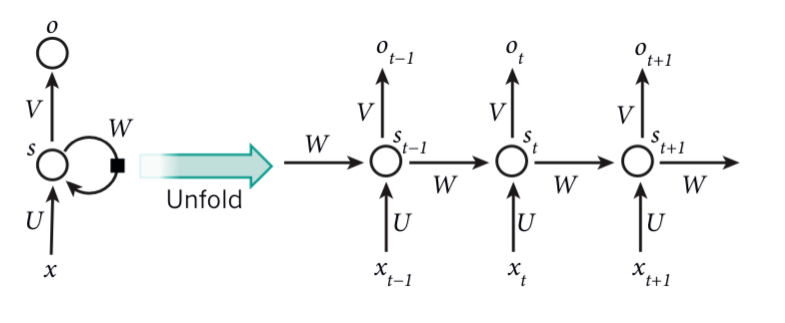
\includegraphics[scale=0.3]{png/RNN.png}
    \caption{A vanilla RNN, image used from \cite{3-deeplearning}}
    \label{fig:RNN}
\end{figure}


\subsubsection{Limitation} 
Training RNNs has proved to be difficult because the backpropagated gradients
either grow or shrink at each time step, so when process sequences
that are very long, RNN is prone to problems such as gradient exploding and
gradient vanishing\cite{3-deeplearning}. 

\subsection{Long Short-Term Memory (LSTM) }

Long Short-Term Memory (LSTM) is a variant of RNN, it was introduced in
\cite{4-lstm}, it has been proved to be a better successor of RNN in learning
long-range temporal data, it
mainly solved the vanishing gradients problem during long sequence training in
RNN.
Simply put, compared to vanilla RNNs, LSTM can perform better in in learning
long-term dependencies. Other than allow previous outputs to be used as current
inputs while having hidden
states in RNN. LSTM adds a method that can transmit information with multiple
timesteps apart. Think of a conveyor belt/carry track running together when you
process the sequences. The information of each node in sequence can be put on
the conveyor belt, or taken off from the conveyor belt, of course, you can also
update the information on the conveyor belt. In this way, the information long
ago is preserved and the loss of information is prevented.

To be exact, the main units of LSTM are introduced in \cite{4-lstm} and
\cite{5-forgetgate} and the illustrative diagram of a LSTM unit is shown in
Fig.\ref{fig:forgetgate} :
\begin{itemize}
	\setlength{\itemsep}{1pt}
	\setlength{\parskip}{0pt}
	\setlength{\parsep}{0pt}
  \item A central unit called Constant error carousel (CEC), which allows for
constant error flow
through special self connected units.
  \item Three gates/multiplicative units that control the flow in CEC;
  \begin{itemize}
 		\item Input gate: prevents CEC from receive irrelevant inputs; 
		\item Forget gate: the mechanism is introduced in \cite{5-forgetgate} that
allow LSTM to "forget" or abandon old and no longer relevant content in
memory.
 		\item Output gate prevents other units receive disturbing information from
CEE;
	\end{itemize}
\end{itemize}


\begin{figure}[htb]
	    \centering
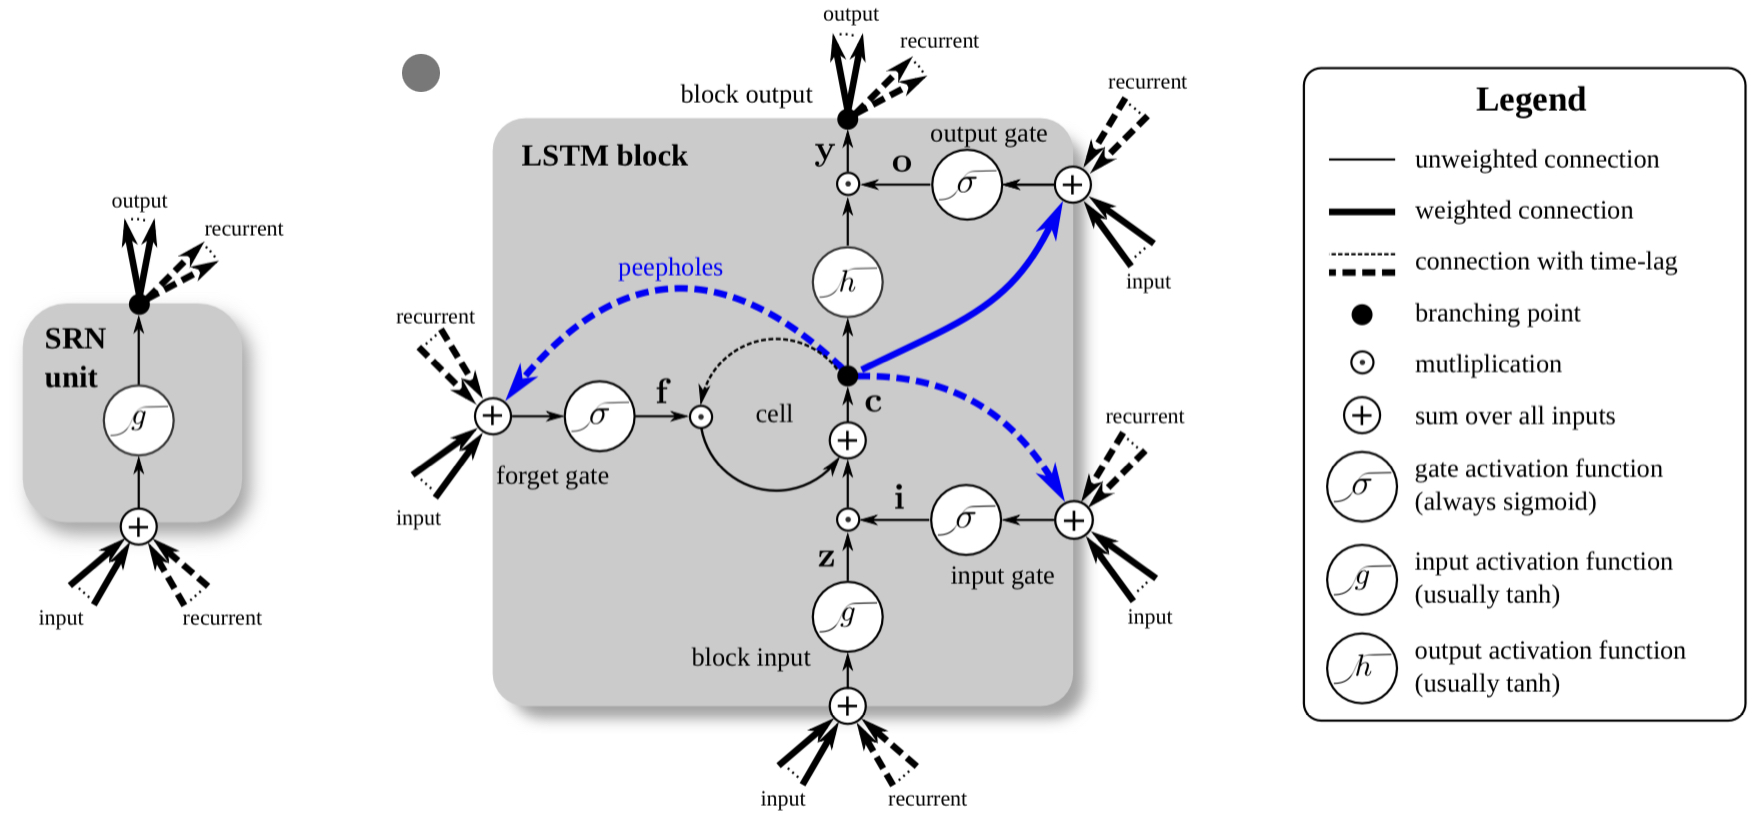
\includegraphics[scale=0.142]{png/forgetgate.png}
    \caption{LSTM with forget gate compare with a simple recurrent network
(SRN), image used from \cite{6-forgetgategraph}}
    \label{fig:forgetgate}
\end{figure}


\subsection{Selected Paper}

The suitable paper selected to match the subject is Akash Singh's master thesis
\cite{7-lstmthisis}. He is a ML Engineer/Data Scientist; Master in Data Science
from KTH Information and Communication Technology. He used an unsupervised
approach to accomplish Long short-term memory (LSTM) technique for anomaly
detection in time series data since the data are unlabelled. 

A RNN model with LSTM units was trained to learn the normal temporal patterns
and predict values in future time steps. The anomaly scores is given by
modelling prediction error result; therefore determine whether a instance is an
anomaly or not. Singh also explored different ways to maintain state in LSTM,
and the effect of different number of time steps used on prediction and
detection performance.

Three real-world datasets were used in his experiments, the results show that
maintaining LSTM state is critical for getting proper result, LSTM RNNs are
suitable for general purpose time series modelling and anomaly detection.

\subsection{Contribution}

TBA 

\section{Methods, Network Architecture, Datasets and File Directories}

Singh's experiments and model was written and implemented using Python
programming language with Keras; His algorithm contains two parts. Part one is
to train a prediction model by learning normal temporal patterns from dataset,
the model can predict future time series. Part two is the anomaly detection,
anomaly scores are computed from the prediction errors.


\subsection{Prediction Model}
The term $lookback$ number and $lookahead$ number were used in 
the model as input the most recent $p$ value and output $q$ value respectively.

The network contains hidden recurrent layer/layers followed by an output
layer. The number of hidden recurrent layers and units are vary for different
dataset. Two recurrent layers are fully connected with each other. To avoid
overfitting $dropout$ is used between two recurrent layers. The output layer is
a fully connected dense NN layer. The number of neuron nodes in the output
layer is equal to the $lookahead$ value, with one neuron for each future value
predicted. Since the model is used for regression, linear activation is used in
the output layer and mean-square error(MSE) as the loss function
\cite{7-lstmthisis}.

The main purpose of the prediction model is to predict multiple time steps
ahead, that is, predicting multiple future values; With a $lookahead$ of $q$ at
time $t$ the model predicts the next $q$ future values i.e.
$t$+1, $t$+2..., $t$+q. Consider a time series with a scale of 10 minutes.
Predicting $lookahead$ value of 6 can give us the behaviour
of the time series for next 30 minutes. It is useful for a system to predict
possible unusual behaviour, e.g. an extreme value, early alerts can be sent
out. 

\subsection{Anomaly Detection and Data Pre-processing}
The prediction errors is used as anomaly indicators, which
is the difference between prediction made at time step $t$-1 and the input
value received at current time step $t$. 

The prediction errors from training data are modelled using a Gaussian
distribution; the mean and variance are computed
using maximum likelihood estimation (MLE). 

On new data, the log probability densities (PDs) of errors are calculated and
used as anomaly scores: the lower the PD values the greater likelihood of the
instance being an anomaly.

A validation set contains both normal instances and anomalies is used to set a
threshold on log PD values; it can separate anomalies from normal
instances and produce as few false positive errors as possible. Finally, a
separate test set containing both normal instances and anomalies is used to
evaluate the model.

In order to learn normal time series patterns and optimise prediction
performance, only normal data without anomalies is used for training LSTM RNN
model. For different dataset, each is divided into four subsets: a
training set, $N$, with only normal values; validation set, $V_N$, with
only
normal values; a second validation set, $V_A$, with
normal values and anomalies; and a test set, $T$ , having both normal values
and anomalies.
There are three main procedures of the LSTM RNN training algorithm:
\begin{itemize}
	\setlength{\itemsep}{1pt}
	\setlength{\parskip}{0pt}
	\setlength{\parsep}{0pt}
	\item 1. Set $N$ with only normal values is used for training prediction
model, Bayesian optimization \cite{8-BayesianOp} to find the best values
for network hyper-parameters. And $V_N$ is used for early stopping to prevent
model overfitting.
	\item 2. Gaussian distribution is used for modelling prediction errors on $N$.
The trained prediction model is applied on $V_A$. The log PD of errors are
calculated from $V_A$ and used as anomaly scores. A threshold is set on the log
PD values which separates the possible anomalies from normal values.
	\item 3. The prediction errors from the test set $T$ is used for the set
threshold, therefore it is used as anomaly indicator to identify anomalies from
the test set $T$.
\end{itemize}
Due to the report length constraint, Singh's full algorithm
steps can be viewed in \cite{7-lstmthisis}.


\subsection{Datasets}
Instead of application specific datasets or generate artificial datasets;
Because it is difficult to judge how well an anomaly detection algorithm would
generalize to different type datasets and there is no real-world validity of
the actual anomalies and algorithm performance\cite{7-lstmthisis}. 
To guard against these problems, three real-world data sets were used in
Singh's experiments: Numenta’s Machine
Temperature Dataset, Power Demand Dataset and ECG Dataset. All three datasets
contain real world anomalies annotated by domain experts; And all been used in
previous works on anomaly detection.

\subsection{Code Directories}
The full code of the project is under \path{/Code}. There are four main parts
of the original code that I explored or conduct experiments.

\begin{itemize}
	\setlength{\itemsep}{1pt}
	\setlength{\parskip}{0pt}
	\setlength{\parsep}{0pt}
	\item The configuration of model hyper-parameters is placed under
\path{/Code/configuration/}
	\item The LSTM model implementation is placed under \path{Code/models/}
	\item The LSTM predictor that train model and predict results is
\path{Code/lstm_predictor.py}
	\item The real-world datasets are stored in \path{Code/resources/data/}
\end{itemize}


\section{The Problems and Limitation of Current System}

Singh's model are worked quite well for both Power Demand Dataset and
ECG Dataset (i.e. electrical activity of the heart). According to Singh's
thesis, the model detected all 5 anomalies in  the Power Demand test set with
the PD threshold of −24 but there is 1 small false positive error. For ECG test
set, the model with a threshold of −23 detects all three anomalies with no
error. It is because they all have consistent and repetitive patterns, and the
LSTM model will be relatively easy to learn these pattern.
Fig.\ref{fig:powerdemand} shows example plots of a normal and an anomalous
weekly cycle, the ECG dataset is produce the plot similar to Power Demand
Dataset.

\begin{figure}[htb]
	    \centering
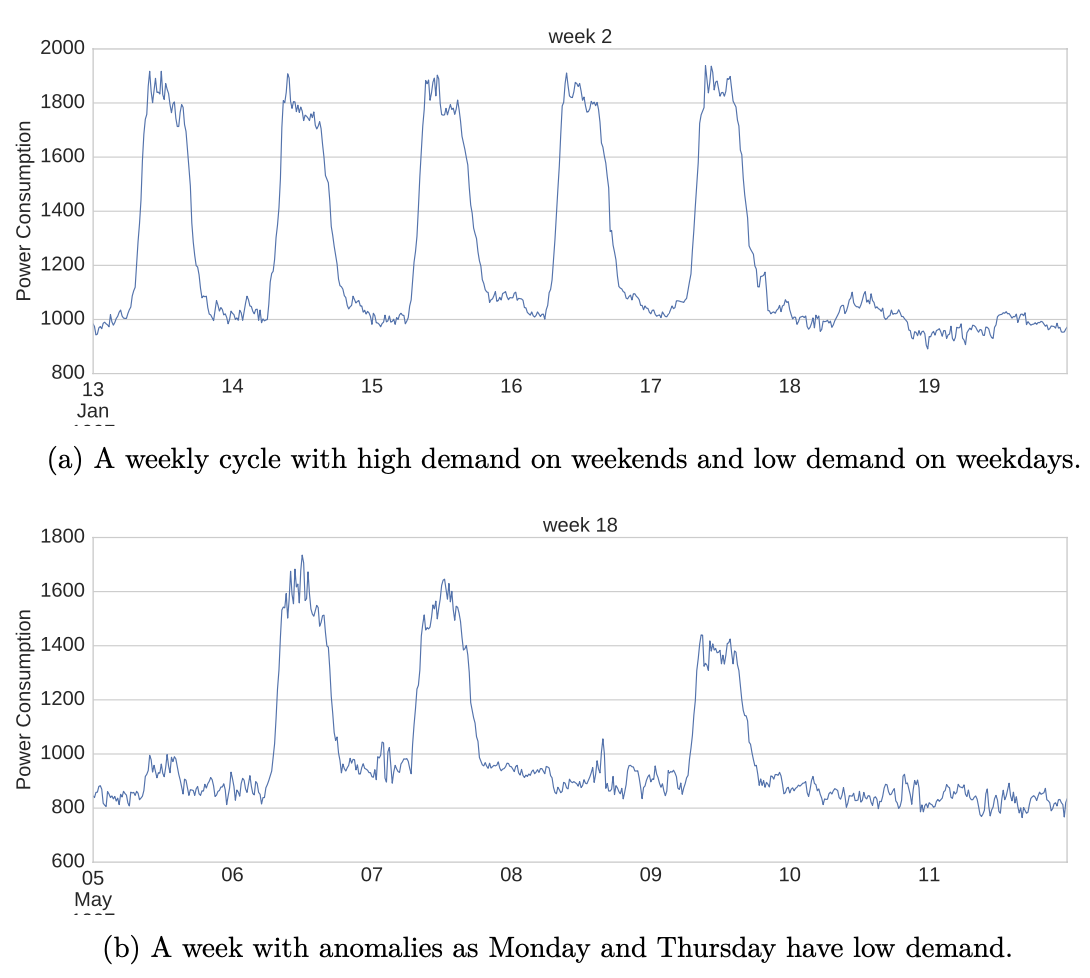
\includegraphics[scale=0.45]{png/powerdemand.png}
    \caption{Power demand normal and anomalous patterns
\cite{7-lstmthisis} }
    \label{fig:powerdemand}
\end{figure}

However, there are four anomalies in the machine temperature dataset, the
results of the anomaly detection on sets $V_A$ and $T$ are shown in
Fig.\ref{fig:o-validationResult}
and Fig/\ref{fig:o-testResult} respectively, orange shaded area in the graph
denotes possible anomalies made by the LSTM algorithm. The PD threshold of −11
was necessary to detect the first anomaly in set $V_A$, but there are quite a
few false positives errors. On T the threshold of −11 detected the second
anomaly but did not detect the first anomaly, and also incurred a few false
positives before the first anomaly.

The result with too many false positives will make the detection unusable. TBA

The machine temperature dataset does not seem to have any repeating
pattern and indeed the performance of the Singh's model was found to be
insensitive to how the state was maintained as he mentioned on the thesis.


\begin{figure}[htb]
	    \centering
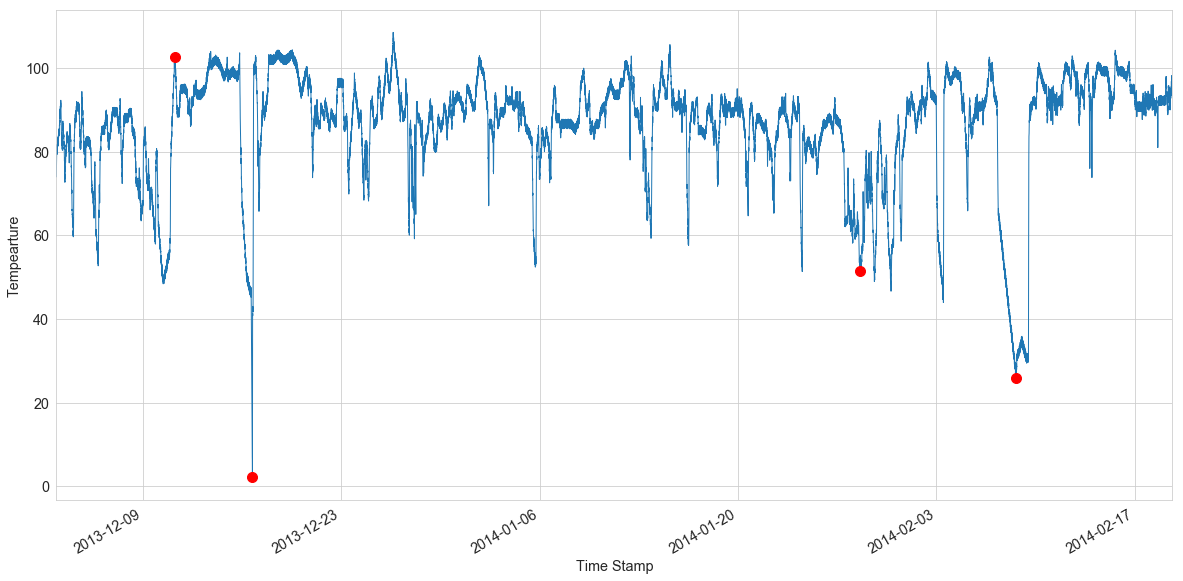
\includegraphics[scale=0.21]{png/o-actualAnomalies.png}
    \caption{Normal pattern/values and actual anomalies in the Numenta’s
Machine
Temperature Dataset}
    \label{fig:actualAnomalies}
\end{figure}



\section{Experiment Result and Contribution}

\begin{figure}[htb]
	    \centering
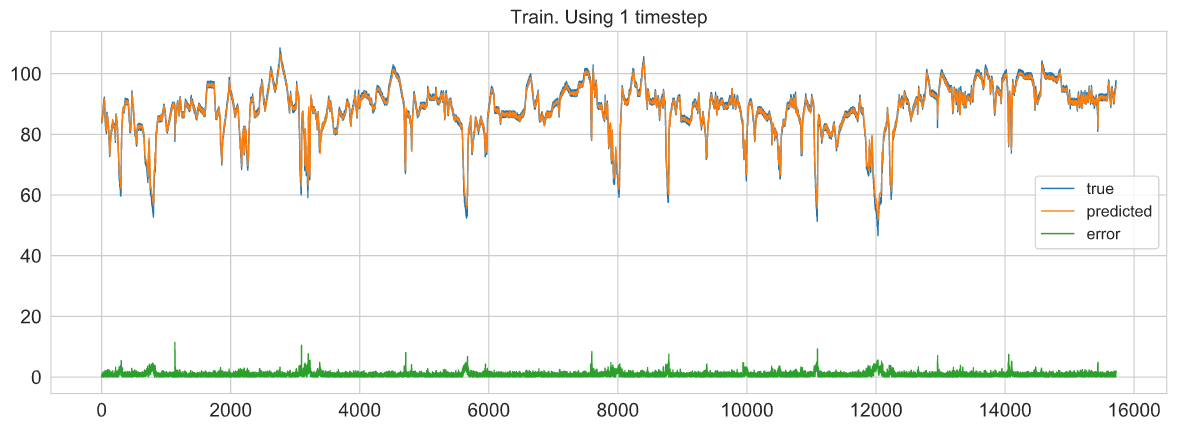
\includegraphics[scale=0.21]{png/m-prediction.png}
    \caption{Prediction result on machine temperature dataset after
modification}
    \label{fig:m-prediction}
\end{figure}

\begin{figure}[htb]
	    \centering
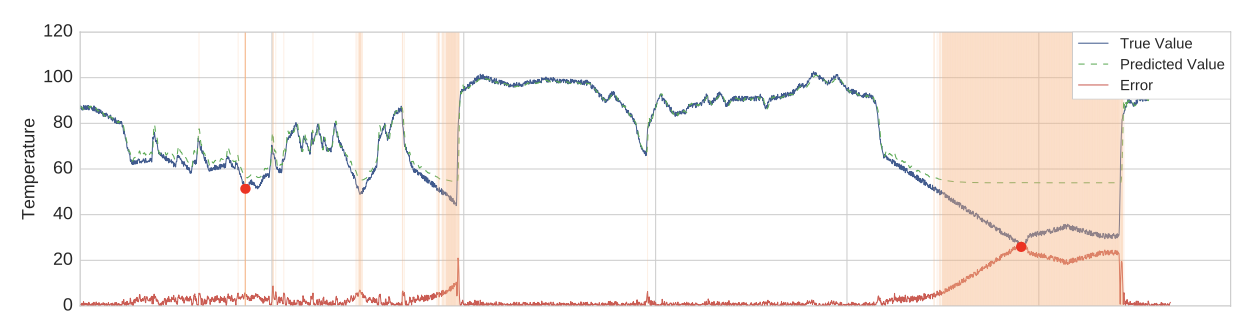
\includegraphics[scale=0.41]{png/o-validationResult.png}
    \caption{Original validation set results on machine temperature dataset}
    \label{fig:o-validationResult}
\end{figure}

\begin{figure}[htb]
	    \centering
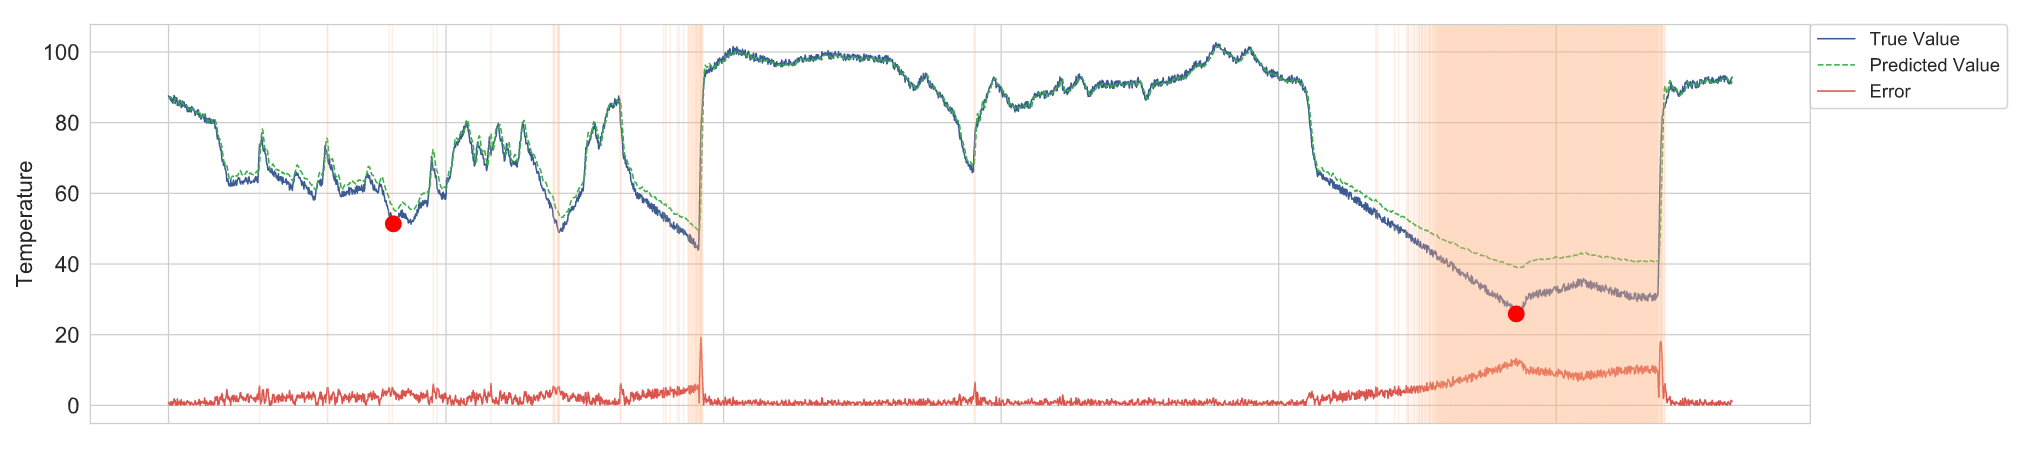
\includegraphics[scale=0.28]{png/m-validationResult.png}
    \caption{Validation set results on machine temperature dataset after
modification}
    \label{fig:m-validationResult}
\end{figure}

\begin{figure}[htb]
	    \centering
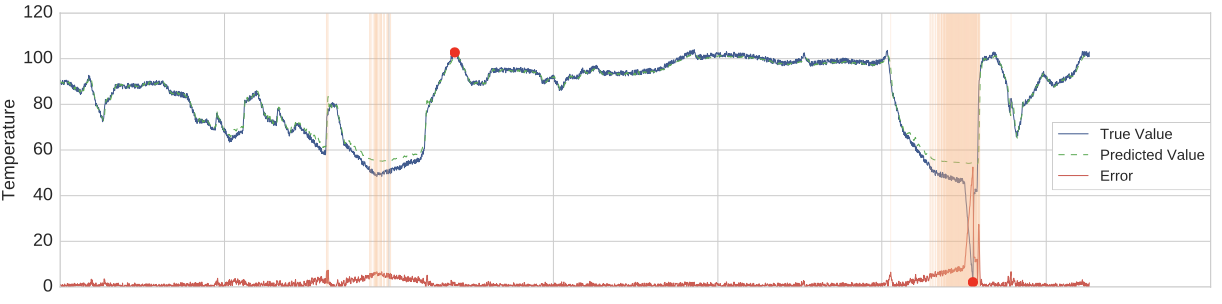
\includegraphics[scale=0.42]{png/o-testResult.png}
    \caption{Original test set results on machine temperature dataset}
    \label{fig:o-testResult}
\end{figure}

\begin{figure}[htb]
	    \centering
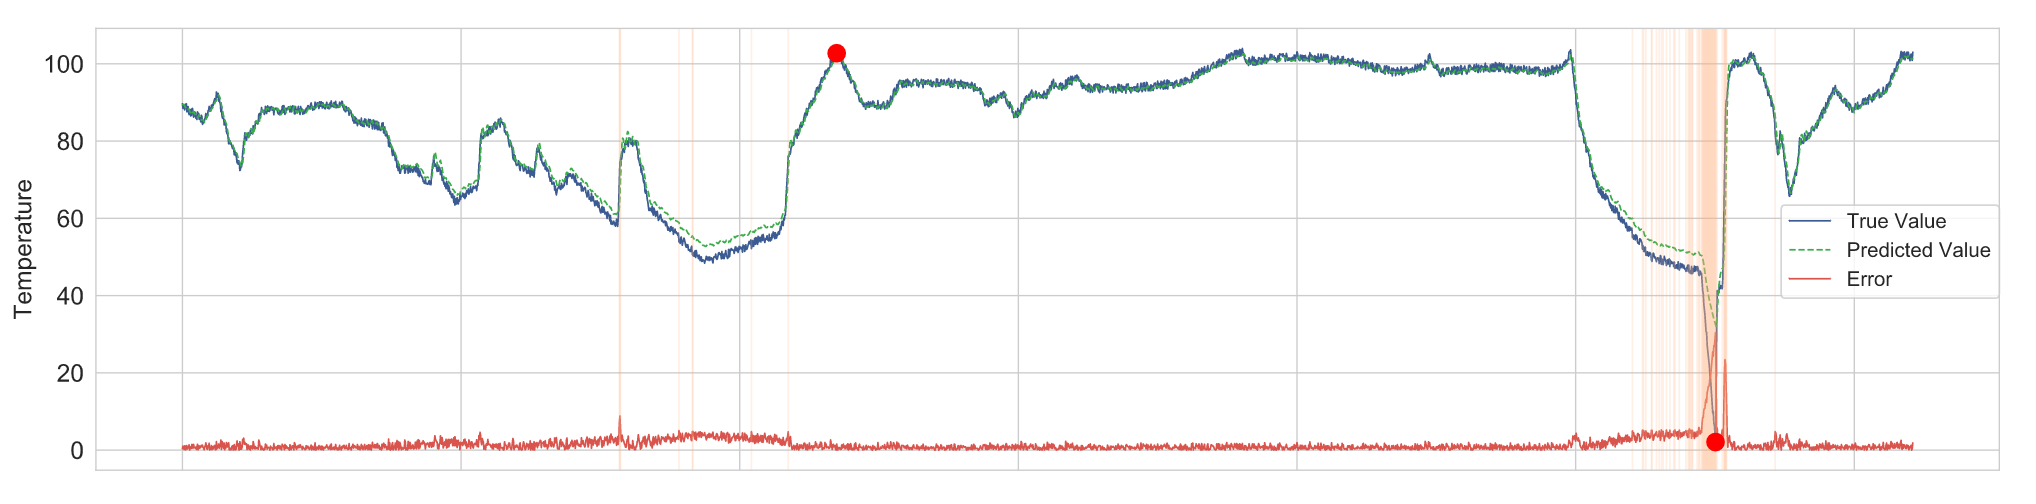
\includegraphics[scale=0.26]{png/m-testResult.png}
    \caption{Test set results on machine temperature dataset after
modification}
    \label{fig:m-testResult}
\end{figure}


\section{Conclusion}



\clearpage
%\vfill\pagebreak
%\vfill\pagebrea


% References should be produced using the bibtex program from suitable
% BiBTeX files (here: strings, refs, manuals). The IEEEbib.bst bibliography
% style file from IEEE produces unsorted bibliography list.
% -------------------------------------------------------------------------
\bibliographystyle{IEEEbib}
\bibliography{refs}

\end{document}
